\documentclass[tikz,border=2pt]{standalone}
\usepackage{amsmath,amssymb}
\usepackage{pgfplots}
\pgfplotsset{compat=1.18}

\begin{document}
% Unit balls {||x||_p <= 1} in R^2: a diamond for p=1, a circle for p=2, a rounded square for p=4,
% the square for p=∞. Larger p gives a larger ball.
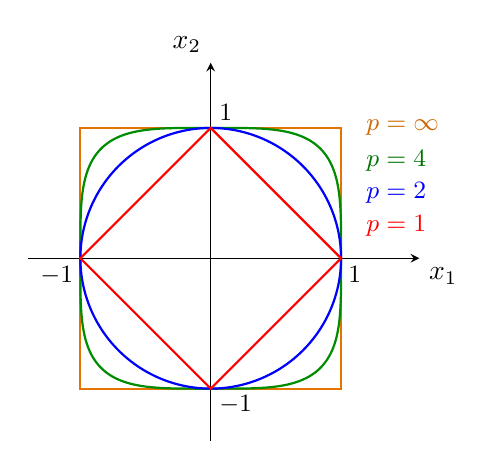
\begin{tikzpicture}
	\begin{axis}[
		axis lines=middle, axis equal image,
		xmin=-1.4, xmax=1.6, ymin=-1.4, ymax=1.5,
		xtick=\empty, ytick=\empty,
		xlabel={$x_1$}, ylabel={$x_2$},
		xlabel style={below right}, ylabel style={above left},
		samples=200, smooth, clip=false, width=7.4cm
		]
		\draw[thick, orange!90!black] (axis cs:-1,-1) rectangle (axis cs:1,1);
		\addplot[thick, green!55!black, domain=0:360, samples=240] ({sign(cos(x))*abs(cos(x))^0.5}, {sign(sin(x))*abs(sin(x))^0.5});
		\addplot[thick, blue, domain=0:360, samples=120] ({cos(x)}, {sin(x)});
		\draw[thick, red] (axis cs:1,0) -- (axis cs:0,1) -- (axis cs:-1,0) -- (axis cs:0,-1) -- cycle;
		\node[anchor=north west, font=\small, inner sep=1.5pt] at (axis cs:1.02,-0.03) {$1$};
		\node[anchor=north east, font=\small, inner sep=1.5pt] at (axis cs:-1.02,-0.03) {$-1$};
		\node[anchor=south west, font=\small, inner sep=1.5pt] at (axis cs:0.03,1.02) {$1$};
		\node[anchor=north west, font=\small, inner sep=1.5pt] at (axis cs:0.03,-1.02) {$-1$};
		\node[orange!80!black, anchor=west, font=\small] at (axis cs:1.12,1.0) {$p=\infty$};
		\node[green!45!black, anchor=west, font=\small] at (axis cs:1.12,0.75) {$p=4$};
		\node[blue, anchor=west, font=\small] at (axis cs:1.12,0.5) {$p=2$};
		\node[red, anchor=west, font=\small] at (axis cs:1.12,0.25) {$p=1$};
	\end{axis}
\end{tikzpicture}
\end{document}
